\documentclass[a4paper,10pt]{article}

\usepackage{amsmath}
\usepackage{amsfonts}
\usepackage{color}
\usepackage[pdftex]{graphicx}

\usepackage{color}%[dvips]
\definecolor{darkgreen}{rgb}{0.1,0.5,0.1}
\definecolor{darkblue}{rgb}{0.0,0.0,0.5}
\definecolor{mygrey}{rgb}{0.29,0.29,0.29}
\usepackage{hyperref}
\hypersetup{colorlinks,%
                citecolor=darkgreen,%
%               filecolor=black,%
                linkcolor=darkblue,%
%               urlcolor=black,%
                pdftex}

\usepackage[square,numbers]{natbib}

\newcommand{\todo}{\textcolor{red}{TODO: }}

\newcommand{\bs}[1]{\mathbf{#1}}					% bold symbol
\newcommand{\bgs}[1]{\boldsymbol{#1}}				% bold greek symbol
\newcommand{\ud}{\mathrm{d}}					% derivative
\newcommand{\pd}[2]{\frac{\partial #1}{\partial #2}} 	% partial derivative
\newcommand{\ppd}[3]{\frac{\partial^2 #1}{\partial #2 \partial #3}} % 2nd order partial derivative
\newcommand{\tr}{\mathsf{T}}				% transpose, also possible: \top
\newcommand{\eq}[1]{\begin{equation} #1 \end{equation}}% equation environment
\newcommand{\trace}[1]{\mathrm{Tr}\left(#1\right)}					% trace

\newcommand{\gc}[1]{\tilde{#1}} % generalised coordinates
\renewcommand{\ss}{u}         % scalar time dependent (state) variable
  \newcommand{\sz}{z}         % scalar state variable
  \newcommand{\sv}{v}         % scalar output variable
  \newcommand{\so}{y}         % scalar observed variable
  \newcommand{\sh}{x}         % scalar hidden variable
  \newcommand{\st}{s}         % scalar combined state variable
  \newcommand{\spe}{\epsilon} % scalar prediction error
  \newcommand{\spm}{\mu}    % scalar posterior mode
  \newcommand{\sog}{\gc{\so}}         % scalar observed variable generalised
  \newcommand{\szg}{\gc{\sz}}         % scalar state variable generalised
  \newcommand{\svg}{\gc{\sv}}         % scalar output variable generalised
  \newcommand{\speg}{\gc{\spe}} % scalar prediction error generalised
\renewcommand{\sp}{\theta}    % scalar parameter
  \newcommand{\ps}{\bs{\ss}}    % vector  time dependent (state) variable
  \newcommand{\pz}{\bs{\sz}}    % vector state variable
  \newcommand{\pv}{\bs{\sv}}    % vector output variable
  \newcommand{\po}{\bs{\so}}    % vector observed variable
  \newcommand{\ph}{\bs{\sh}}    % vector hidden variable
  \newcommand{\pt}{\bs{\st}}     % vector combined state variable
  \newcommand{\ppe}{\bgs{\spe}} % vector prediction error
  \newcommand{\ppm}{\bgs{\spm}}   % vector posterior mode
  \newcommand{\psg}{\gc{\ps}}    % vector  time dependent (state) variable generalised
  \newcommand{\pzg}{\gc{\pz}}    % vector state variable generalised
  \newcommand{\pvg}{\gc{\pv}}    % vector output variable generalised
  \newcommand{\ptg}{\gc{\pt}}     % vector combined state variable generalised
  \newcommand{\pog}{\gc{\po}}    % vector observed variable generalised
  \newcommand{\phg}{\gc{\ph}}    % vector hidden variable generalised
  \newcommand{\ppeg}{\gc{\ppe}} % vector prediction error
  \newcommand{\ppmg}{\gc{\ppm}} % vector posterior mode generalised
  \newcommand{\pp}{\bgs{\sp}} % vector parameter
  \newcommand{\Ps}{\bs{U}}    % matrix  time dependent (state) variable
  \newcommand{\Po}{\bs{Y}}    % matrix observed variable
  \newcommand{\Pv}{\bs{V}}    % matrix output variable
  \newcommand{\Ph}{\bs{X}}    % matrix hidden variable
  \newcommand{\Pt}{\bs{S}}    % matrix combined state variable

\newcommand{\D}{\bs{D}}				% differential operator
\newcommand{\K}{\bs{K}}					% kernel
\newcommand{\E}[2][]{\left\langle #2 \right\rangle_{#1}}	% expectation
\newcommand{\Ent}{\mathrm{H}}			% entropy
\newcommand{\U}{\mathrm{U}}			% internal energy
\newcommand{\Ua}{\bar{\mathrm{U}}}		% internal action
\newcommand{\V}{\mathrm{V}}			% variational energy
\newcommand{\Va}{\bar{\mathrm{V}}}		% variational action
\newcommand{\N}{\mathcal{N}}			% Gaussian distribution
\newcommand{\F}{\mathcal{F}}				% (Laplace) approximated free energy
\newcommand{\Fa}{\bar{\mathcal{F}}}		% approximated free action
\newcommand{\R}{\mathbb{R}}				% real numbers
\newcommand{\Cov}{\bgs{\Sigma}}			% covariance
\renewcommand{\det}[1]{\mathrm{det}(#1)}	% determinant
%\renewcommand{\det}[1]{|#1|}	% determinant

%opening
\title{Deriving Friston's DEM}
\author{Sebastian Bitzer \and Burak I. Yildiz}

\begin{document}

\maketitle

\begin{abstract}
In recent years Karl Friston has prominantly promoted his idea of free energy in the neurosciences. Although there it is highly received, many more technically minded scientists are a bit astranged, because his technical arguments are hard, or impossible, to follow.

Friston's free energy principle has two sides: 1) filtering for estimating hidden states in a hierarchical model and 2) control by performing actions which minimise the discrepancy between expectations and observations. In more general terms we can call these 1) perception and 2) action. Here, we want to shed some light on the technical details of 1). These have been presented in \cite{Friston2008a,Friston2008} in the difficult Fristonian way. We will try to fill in the gaps while maintaining a consistent mathematical formulation. As this is partly an interpretation of the Fristonian descriptions we do not guarantee to represent his ideas completely, but we hope to provide a formulation which is more accessible to mathematically minded researchers. Also, this report should be seen as a work-in-progress and possible corrections and clarifications are welcome.
\end{abstract}

\newpage
\tableofcontents

\section{Nonlinear Gaussian Dynamic Models}
Whatever function is used in the end to find the posterior mode, all corresponding gradients are computed from the gradients of $\Ua$. So it is time to look at the structure of $\Ua$. Notice that from here on subscripts of variables or functions are used solely to identify different variables or functions, or to index into matrices and vectors. Partial derivatives are written out in the standard format. While this clutters the formulae more, it helps us to make them conceptually clearer.

First, remember that (eq. \ref{eq:intAction})
\[
    \Ua(\Po,\Ps,\pp) = \log p(\pp) + \int_{t=0}^T \log p(\po(t),\ps(t)|\pp)dt.
\]
The parameter prior, as all other model densities, is chosen to be Gaussian $p(\pp)\sim \N(\bgs{\eta}_\sp,\bgs{\Psi}^\sp)$ such that 
\begin{align}
    \log p(\pp) &= -\frac{1}{2}(\pp - \bgs{\eta}_\sp)^\tr\bgs{\Psi}^{\sp^{-1}}(\pp - \bgs{\eta}_\sp) + c\\
    &= -\frac{1}{2}\ppe_\sp^\tr\bgs{\Pi}^{\sp}\ppe_\sp + c
\end{align}
where we have lumped terms from the normalisation constant of the Gaussian distribution into the constant $c$ and introduced Friston's prediction error - precision formulation in the second line.

The joint data - state density is a bit more difficult. The probabilistic definition is
\eq{
    p(\po(t),\ps(t)|\vec{\Po}(t),\pp) = p(\po(t)|\ps(t),\pp)p(\ps(t)|\vec{\Po}(t),\pp)
}
where $\vec{\Po}(t)$ is all data observed previous to time $t$.

The observation density $p(\po(t)|\ps(t),\pp)$ can be defined in a straightforward way based on an output nonlinearity with additive zero-mean Gaussian noise: $g(\ps(t),\pp)+\bgs{\omega}_\so$, $\bgs{\omega}_\so\sim \N(\bs{0},\bgs{\Psi}^\so)$ such that
\begin{align}
    \log p(\po(t)|\ps(t),\pp) &= -\frac{1}{2}(\po(t) - g(\ps(t),\pp))^\tr\bgs{\Psi}^{\so^{-1}}(\po(t) - g(\ps(t),\pp)) + c\\
    &= -\frac{1}{2}\ppe_\so^\tr\bgs{\Pi}^{\so}\ppe_\so + c.
\end{align}
The prior $p(\ps(t)|\vec{\Po}(t),\pp)$ is most generally defined as
\eq{
    p(\ps(t)|\vec{\Po}(t),\pp) = \E[\vec{\Ps}(t)]{p(\ps(t),\vec{\Ps}(t)|\vec{\Po}(t),\pp)}
}
which states that the prior for the state at time $t$ depends on the observations previous to $t$ $\vec{\Po}(t)$ via averaging over all posterior state trajectories previous to $t$. Such a model is intractable. So we use a Markov assumption to make the current state only depend on the previous
\begin{align}
    p(\ps(t)|\vec{\Po}(t),\pp) &= \E[\vec{\ps}(t)]{p(\ps(t),\vec{\ps}(t)|\vec{\Po}(t),\pp)}\\
    &= \label{eq:statePrior} \E[\vec{\ps}(t)]{p(\ps(t)|\vec{\ps}(t),\pp)p(\vec{\ps}(t)|\vec{\Po}(t),\pp)}.
\end{align}
Well, at least this is what you would do in a discrete time setting where the current state is related to a previous state via $\ps(t) = f(\vec{\ps}(t),\pp)$. In the continuous time setting we only have the functional relationship
\eq{
    \dot{\ps} = f(\ps,\pp)
}
and we have to solve this differential equation to get $\ps(t)$ for the observation density. Friston introduced generalised states to overcome this problem. 

\subsection{Generalised Coordinates}
A generalised state represents the future trajectory of a state in form of an infinitely large vector containing its time derivatives
\eq{
    \psg(t) = \left[\begin{array}{c} \ps(t)\\ \pd{\ps(t)}{t}\\ \ppd{\ps(t)}{t}{t}\\ \vdots \end{array}\right] = \left[\begin{array}{c} \ps\\ \dot{\ps}\\ \ddot{\ps}\\ \vdots \end{array}\right].
}
This can also be applied to functions which depend on time-varying variables
\eq{\label{eq:gcf}
    \gc{\bs{f}}(\psg(t),\pp) = \left[\begin{array}{c} f(\ps(t),\pp)\\ \pd{f(\ps(t),\pp)}{t}\\ \ppd{f(\ps(t),\pp)}{t}{t}\\ \vdots \end{array}\right] \approx \left[\begin{array}{c} f(\ps(t),\pp)\\ \pd{f(\ps(t),\pp)}{\ps}\pd{\ps}{t}\\ \pd{f(\ps(t),\pp)}{\ps}\ppd{\ps}{t}{t}\\ \vdots \end{array}\right] = \left[\begin{array}{c} f(\ps(t),\pp)\\ f_\ps\dot{\ps}\\ f_\ps\ddot{\ps}\\ \vdots \end{array}\right]
}
\eq{
    \gc{\bs{g}}(\psg(t),\pp) = \left[\begin{array}{c} g(\ps(t),\pp)\\ \pd{g(\ps(t),\pp)}{t}\\ \ppd{g(\ps(t),\pp)}{t}{t}\\ \vdots \end{array}\right] \approx \left[\begin{array}{c} g(\ps(t),\pp)\\ \pd{g(\ps(t),\pp)}{\ps}\pd{\ps}{t}\\ \pd{g(\ps(t),\pp)}{\ps}\ppd{\ps}{t}{t}\\ \vdots \end{array}\right] = \left[\begin{array}{c} g(\ps(t),\pp)\\ g_\ps\dot{\ps}\\ g_\ps\ddot{\ps}\\ \vdots \end{array}\right]
}
where we have assumed that $f$ and $g$ are locally linear with respect to $\ps$. 


\subsection{Dynamic Model in Generalised Coordinates}
It is then possible to redefine the observation density in generalised coordinates and obtain
\begin{align}
    \log p(\pog(t)|\gc{\bs{g}}(t),\pp) &= -\frac{1}{2}(\pog(t) - \gc{\bs{g}}(\psg(t),\pp))^\tr\gc{\bgs{\Psi}}^{\so^{-1}}(\pog(t) - \gc{\bs{g}}(\psg(t),\pp)) + c\\
    &= -\frac{1}{2}\ppeg_\so^\tr\gc{\bgs{\Pi}}^{\so}\ppeg_\so + c.
\end{align}
Equivalently, we can now define the state transition probability in generalised coordinates based on the differential equation with additive Gaussian noise $\D\psg(t) = \gc{\bs{f}}(\psg(t),\pp)+\gc{\bgs{\omega}}_\ss$, $\gc{\bgs{\omega}}_\ss\sim \N(\bs{0},\gc{\bgs{\Psi}}^\ss)$ to get
\begin{align}
    \log p(\D\psg(t)|\gc{\bs{f}}(t),\pp) &= -\frac{1}{2}(\D\psg(t) - \gc{\bs{f}}(\psg(t),\pp))^\tr\gc{\bgs{\Psi}}^{\ss^{-1}}(\psg(t) - \gc{\bs{f}}(\psg(t),\pp)) + c\\
    &= -\frac{1}{2}\ppeg_\ss^\tr\gc{\bgs{\Pi}}^{\ss}\ppeg_\ss + c
\end{align}
where $\D$ is a differential operator which shifts the corresponding generalised coordinates up by one coordinate such that
\eq{\label{eq:derivativeOperator}
    \D\psg = \left[\begin{array}{c} \dot{\ps}\\ \ddot{\ps}\\ \vdots \end{array}\right].
}
We can now identify $p(\D\psg(t)|\gc{\bs{f}}(t),\pp)$ with $p(\ps(t)|\vec{\ps}(t),\pp)$ from eq. \eqref{eq:statePrior}. Thus a full probabilistic model would integrate over $\gc{\bs{f}}(t)$:
\eq{
    p(\D\psg(t)|\vec{\Po}(t),\pp) = \E[p(\gc{\bs{f}}(t)|\vec{\Po}(t),\pp)]{p(\D\psg(t)|\gc{\bs{f}}(t),\pp)}.
}
Unfortunately, we don't know the distribution $p(\gc{\bs{f}}(t)|\vec{\Po}(t),\pp)$. The variational approximation gives us a Gaussian $q(\psg(t))$, but computing $\gc{\bs{f}}(t) = \gc{\bs{f}}(\psg(t),\pp)$ via eq. \eqref{eq:gcf} transforms $\psg(t)$ nonlinearly. Friston uses the simplest possible approximation: a point estimate by (implicitly) setting $p(\gc{\bs{f}}(t)|\vec{\Po}(t),\pp)$ to the Dirac delta function at the current estimate $\gc{\bgs{\mu}}_{\gc{f}}(t)$ of $\gc{\bs{f}}(t)$, i.e.,
\eq{
    p(\gc{\bs{f}}(t)|\vec{\Po}(t),\pp) \approx \delta(\gc{\bs{f}}(t) - \gc{\bgs{\mu}}_{\gc{f}}(t))
}
such that
\eq{
    \E[p(\gc{\bs{f}}(t)|\vec{\Po}(t),\pp)]{p(\D\psg(t)|\gc{\bs{f}}(t),\pp)} \approx p(\D\psg(t)|\gc{\bgs{\mu}}_{\gc{f}}(t),\pp).
}
This approximation has an important impact on the inference. It means that state uncertainty is not propagated through time, i.e., the posterior covariances of the states only depend on the prior covariances $\gc{\bgs{\Psi}}^\ss$ and $\gc{\bgs{\Psi}}^\so$ and on the corresponding functions $f$ and $g$. On the one hand, this prevents the divergence of state uncertainty over time through accumulation of errors. On the other hand, it also prevents posterior uncertainty to decrease, for example, when the dynamics prescribed by the model can be followed accurately over an extended period of time. In any case, it makes the posterior covariances of the states purely instantaneous measures of uncertainty which do not necessarily reflect the true uncertainties accumulated over time.


\subsection{Generalised Covariances}
We used "generalised covariances" to define the Gaussian densities above, i.e., we introduced covariances for the representations in generalised coordinates. To this point, it is still unclear to us how Friston derived his formula for computing generalised covariances. However, this is central to the definition of his probabilistic model as it defines what kind of stochastic process he assumes. We now state what he suggests and comment on his equations as far as we understand them. 

He defines generalised covariances as\footnote{Friston actually defines generalised precisions instead of generalised covariances, but this turns out the same, because $(\bs{A}\otimes\bs{B})^{-1} = \bs{A}^{-1}\otimes\bs{B}^{-1}$, if $\bs{A}$ and $\bs{B}$ are invertible.}
\eq{
    \gc{\bgs{\Psi}} = \bs{S}(\gamma) \otimes \bgs{\Psi}
}
where $\bs{S}(\gamma)$ is a potentially infinitely large (depending on the number of considered generalised coordinates) matrix which translates an assumed covariance for a state $\ps$ $\bgs{\Psi}$ to the covariances for its generalised coordinates $\dot{\ps}, \ddot{\ps}, \dots$ by scaling (and mixing) $\bgs{\Psi}$. Friston states that the "temporal covariance" $\bs{S}(\gamma)$ can be written as
\eq{
    \bs{S}(\gamma) = \left[\begin{array}{cccc} 1 & 0 & \ddot{\rho}(0) & \cdots\\
0 & - \ddot{\rho}(0) & 0 &\\
 \ddot{\rho}(0) & 0 & \ddot{\ddot{\rho}}(0) & \\
\vdots & & & \ddots
\end{array}\right]
}
where $\rho(\Delta t)$ is the autocorrelation function of the noise and $\ddot{\rho}(0)$ its second derivative with respect to time evaluated at $\Delta t = 0$. The origin of this relationship is a mystery to us. That $\rho$ only has a single argument hints at the assumption of a stationary noise process, but the derivative of the corresponding autocorrelation function with respect to time should be 0 then, because it would not change with time. Friston further states that, if $\rho$ is a Gaussian with variance $\gamma$, then
\eq{
    \bs{S}(\gamma) = \left[\begin{array}{cccc} 1 & 0 & -\frac{1}{2\gamma} & \cdots\\
0 & \frac{1}{2\gamma} & 0 &\\
-\frac{1}{2\gamma} & 0 & \frac{3}{4\gamma^2} & \\
\vdots & & & \ddots
\end{array}\right],
}
but the elements of $\bs{S}(\gamma)$ here are certainly not the derivatives of a Gaussian. 

Consequently, we are tapping completely in the dark when trying to interpret generalised covariances. Why, for example, does a state only covary with every second of its generalised coordinates (cf. nonzero entries in $\bs{S}(\gamma)$)? We can only say for sure that the generalised covariance increases for higher order coordinates as long as $\gamma$ is small enough. In his code, Friston sets $\gamma = 1/4$ by default which means that the generalised covariances quickly become so large for higher order coordinates that these coordinates become completely uninformative and considering more than 6, or so, is a waste of computing time.


\subsection{Internal Action of Dynamic Model}
To summarise, we can now rewrite the internal action in terms of prediction errors and precisions
\begin{align}
    \Ua(\Po,\Ps,\pp) &= \log p(\pp) + \int_0^T \log p(\pog(t),\psg(t)|\pp)dt\nonumber\\
    &= C - \frac{1}{2}\left(\ppe_\sp^\tr\bgs{\Pi}^{\sp}\ppe_\sp + \int_0^T \ppeg_\so^\tr(t)\gc{\bgs{\Pi}}^{\so}\ppeg_\so(t) + \ppeg_\ss^\tr(t)\gc{\bgs{\Pi}}^{\ss}\ppeg_\ss(t)  dt\right)
\end{align}
with 
\begin{align}
    C &= \frac{1}{2}\log\det{\bgs{\Pi}^{\sp}} - \frac{n_\sp}{2}\log 2\pi\nonumber\\
    &\quad + \frac{1}{2} \int_0^T \log\det{\gc{\bgs{\Pi}}^{\so}} + \log\det{\gc{\bgs{\Pi}}^{\ss}} - (n_\so + n_\ss)\log 2\pi dt\\
    &= \frac{1}{2}\log\det{\bgs{\Pi}^{\sp}} - \frac{n_\sp}{2}\log 2\pi\nonumber\\
    &\quad + \frac{T}{2} \left( \log\det{\gc{\bgs{\Pi}}^{\so}} + \log\det{\gc{\bgs{\Pi}}^{\ss}} - (n_\so + n_\ss)\log 2\pi \right)
\end{align}
which may potentially depend on $\pp$ and
\begin{align}
    \ppe_\sp &= \pp - \bgs{\eta}_\sp\\
    \ppeg_\so(t) &= \pog(t) - \gc{\bs{g}}(\psg(t),\pp)\\
    \ppeg_\ss(t) &= \D\psg(t) - \gc{\bs{f}}(\psg(t),\pp)
\end{align}
where we have equated $\gc{\bgs{\mu}}_{\gc{f}}=\gc{\bs{f}}$.


\subsection{Hierarchy}
So far we have only considered flat models, but a generalisation to deep, i.e., hierarchical, dynamical models is straightforward. To achieve this we make the model functions on one level depend on the output of the level above. In particular, the model becomes
\eq{\begin{array}{cc}
    \pog(t) = \gc{\bs{g}}^1(\psg^1(t),\pvg^2(t),\pp) + \gc{\bgs{\omega}}_\so & \D\psg^1(t) = \gc{\bs{f}}^1(\psg^1(t),\pvg^2(t),\pp)+\gc{\bgs{\omega}}_{\ss}^1\\
    \pvg^2(t) = \gc{\bs{g}}^2(\psg^2(t),\pvg^3(t),\pp) + \gc{\bgs{\omega}}_\sv^2 & \D\psg^2(t) = \gc{\bs{f}}^2(\psg^2(t),\pvg^3(t),\pp)+\gc{\bgs{\omega}}_{\ss}^2\\
    \vdots & \vdots\\
    \pvg^{l}(t) = \gc{\bs{g}}^l(\psg^l(t),\pvg^{l+1}(t),\pp) + \gc{\bgs{\omega}}_\sv^l & \D\psg^l(t) = \gc{\bs{f}}^l(\psg^l(t),\pvg^{l+1}(t),\pp)+\gc{\bgs{\omega}}_{\ss}^l
\end{array}
}
where we define $\pog(t) = \pvg^{1}(t)$ and $\pvg^{L+1}(t)$ on the top level $L$ is a causal variable which may influence the top level dynamics via direct external input. Note that both $\psg^{l}(t)$ and $\pvg^{l}(t)$ are time-dependent state variables. We call them dynamic variables, $\psg^l(t)$, and output variables, $\pvg^l(t)$, respectively. $\psg^l(t)$ represents the state of the dynamics on level $l$ while $\pvg^l(t)$ represents the output of level $l$ which influences level $l-1$, or corresponds to the observations for $l=1$. 

Because the noise in each level is independent from the noise in the other levels, the internal action becomes\footnote{We here indicate the dependencies of the internal action on both, dynamic and output, variables by replacing $\Po$ with $\Pv$. This conceals a bit the dependence on the observations $\Po$, but it's still correct as $\Po$ is only absorbed into $\Pv$ as first level output variables.}
\begin{align}
    \Ua(\Pv,\Ps,\pp) &= \log p(\pp) + \int_0^T \log p(\pvg^{L+1}(t))\nonumber\\
    &\quad + \sum_{l=1}^L \log p(\pvg^{l}(t),\psg^l(t)|\pvg^{l+1}(t),\pp)dt
\end{align}
where we have introduced the prior probability $p(\pvg^{L+1}(t)) \sim \N(\gc{\bgs{\eta}}_{\sv^{L+1}},\gc{\bgs{\Psi}}^{\sv^{L+1}})$. All other distributions remain Gaussian, too, such that we get
\begin{align}\label{eq:intActionHier}
    \Ua(\Pv,\Ps,\pp) &= C^h  - \frac{1}{2}\ppe_\sp^\tr\bgs{\Pi}^{\sp}\ppe_\sp - \frac{1}{2}\int_0^T \ppeg_{\sv^{L+1}}^\tr(t)\gc{\bgs{\Pi}}^{\sv^{L+1}}\ppeg_{\sv^{L+1}}(t)\nonumber\\
    &\qquad + \sum_{l=1}^L \ppeg_{\sv^l}^\tr(t)\gc{\bgs{\Pi}}^{\sv^l}\ppeg_{\sv^l}(t) + \ppeg_{\ss^l}^\tr(t)\gc{\bgs{\Pi}}^{\ss^l}\ppeg_{\ss^l}(t)  dt
\end{align}
with
\begin{align}
    C^h &= \frac{1}{2}\log\det{\bgs{\Pi}^{\sp}} + \frac{T}{2}\log\det{\gc{\bgs{\Pi}}^{\sv^{L+1}}} - \frac{n_\sp + Tn_{\sv^{L+1}}}{2}\log 2\pi\nonumber\\
    &\quad + \frac{T}{2} \left( \sum_{l=1}^L \log\det{\gc{\bgs{\Pi}}^{\sv^l}} + \log\det{\gc{\bgs{\Pi}}^{\ss^l}} - (n_{\sv^l} + n_{\ss^l})\log 2\pi \right)
\end{align}
and
\begin{align}
    \ppe_\sp &= \pp - \bgs{\eta}_\sp\\
    \ppeg_{\sv^{L+1}}(t) &= \pvg^{L+1}(t) - \gc{\bgs{\eta}}_{\sv^{L+1}}\\
    \ppeg_{\sv^l}(t) &= \pvg^l(t) - \gc{\bs{g}}^l(\psg^l(t),\pvg^{l+1}(t),\pp)\\
    \ppeg_{\ss^l}(t) &= \D\psg^l(t) - \gc{\bs{f}}^l(\psg^l(t),\pvg^{l+1}(t),\pp).
\end{align}


\subsection{Gradients of the Internal Action}


\subsubsection{Gradients with respect to Parameters}
The gradients with respect to parameters obviously depend on what the parameters control. We for now stick with parameterising the functions $\gc{\bs{g}}^l$ and $\gc{\bs{f}}^l$ and consider learning of prior covariances later. Based on \citep[][eq. (85)]{Petersen2008} we get from eq. \eqref{eq:intActionHier}
\begin{align}
    \pd{\Ua(\Pv,\Ps,\pp)}{\pp} &= -\left(\pd{\ppe_\sp}{\pp}\right)^\tr\bgs{\Pi}^{\sp}\ppe_\sp - \int_0^T \sum_{l=1}^L \left(\pd{\ppeg_{\sv^l}(t)}{\pp}\right)^\tr\gc{\bgs{\Pi}}^{\sv^l}\ppeg_{\sv^l}(t)\nonumber\\
    &\quad + \left(\pd{\ppeg_{\ss^l}(t)}{\pp}\right)^\tr\gc{\bgs{\Pi}}^{\ss^l}\ppeg_{\ss^l}(t)  dt
\end{align}
The second order gradients should be of the form (considering a single parameter $\sp_i$ only)
\begin{align}
    \ppd{\frac{1}{2}\ppe_\sp^\tr\bgs{\Pi}^{\sp}\ppe_\sp}{\pp}{\sp_i} &= \pd{}{\sp_i}\left[\left(\pd{\ppe_\sp}{\pp}\right)^\tr\bgs{\Pi}^{\sp}\ppe_\sp\right]\nonumber\\
    &= \left(\ppd{\ppe_\sp}{\pp}{\sp_i}\right)^\tr\bgs{\Pi}^{\sp}\ppe_\sp + \left(\pd{\ppe_\sp}{\pp}\right)^\tr\bgs{\Pi}^{\sp}\pd{\ppe_\sp}{\sp_i}.
\end{align}
However, Friston assumes local linearity such that the second order terms disappear and what remains is (now summarised for all parameters)
\begin{align}
    \ppd{\frac{1}{2}\ppe_\sp^\tr\bgs{\Pi}^{\sp}\ppe_\sp}{\pp}{\pp} &\approx \left(\pd{\ppe_\sp}{\pp}\right)^\tr\bgs{\Pi}^{\sp}\pd{\ppe_\sp}{\pp}.
\end{align}
It would be interesting to know what the advantage is of assuming local linearity of the prediction errors compared to assuming local linearity of $\Ua$ directly, i.e., why not simply ignore second order gradients of $\Ua$ completely? We can test this in the implementation later on. Anyway, the second order gradients of $\Ua$ become
\begin{align}
    \ppd{\Ua(\Pv,\Ps,\pp)}{\pp}{\pp} &\approx -\left(\pd{\ppe_\sp}{\pp}\right)^\tr\bgs{\Pi}^{\sp}\pd{\ppe_\sp}{\pp} - \int_0^T \sum_{l=1}^L \left(\pd{\ppeg_{\sv^l}(t)}{\pp}\right)^\tr\gc{\bgs{\Pi}}^{\sv^l}\pd{\ppeg_{\sv^l}(t)}{\pp}\nonumber\\
    &\quad + \left(\pd{\ppeg_{\ss^l}(t)}{\pp}\right)^\tr\gc{\bgs{\Pi}}^{\ss^l}\pd{\ppeg_{\ss^l}(t)}{\pp}  dt
\end{align}
Notice that any higher order gradients of $\Ua$ with respect to parameters will be 0 under the local linearity assumption for the prediction errors. 


\subsubsection{Gradients with respect to States}
The gradients of the variational energy, e.g., eqs. \eqref{eq:approxVarActionDp} and \eqref{eq:approxVarActionDpp} were defined for all time-dependent variables. This means that we have to combine all states into a long state vector
\eq{
    \ptg(t) = \left[\begin{array}{c}
                     \pvg^2(t)\\
                     \vdots\\
                     \pvg^{L+1}(t)\\
                     \psg^1(t)\\
                     \vdots\\
                     \psg^L(t)
\end{array}\right].
}
Then the variational energy of the parameters from eq. \eqref{eq:approxVarAction} becomes
\eq{
    \Va(\Po,\pp) \approx \Ua(\Po,\gc{\bgs{\mu}}_\Pt,\pp) + \frac{1}{2}\int_0^T \trace{\ppd{\U(\pog(t),\gc{\bgs{\mu}}_{\st(t)},\pp)}{\ptg(t)}{\ptg(t)}\gc{\Cov}^{\st(t)}}dt
}
where we have introduced generalised coordinates and just replaced $\psg$ by $\ptg$ (equivalently for the gradients of the variational energy). We will consider the gradients of the internal action with respect to output, $\pvg^l(t)$, and dynamic variables, $\psg^l(t)$, sequentially. Note that the gradient of the internal action with respect to any particular time-dependent state is equal to the corresponding gradient of the internal energy:
\eq{
    \pd{\Ua(\Pv,\Ps,\pp)}{\pvg^l(t)} = \pd{\U(\pog(t),\ptg(t),\pp)}{\pvg^l(t)}.
}

We are only interested in taking gradients with respect to the \emph{hidden} output variables of levels $l=\{2, \dots, L+1\}$ which are (from eq. \ref{eq:intActionHier})
\begin{align}
    \pd{\U(\pog(t),\ptg(t),\pp)}{\pvg^l(t)} &=  - \left(\pd{\ppeg_{\sv^{l}}(t)}{\pvg^l(t)}\right)^\tr\gc{\bgs{\Pi}}^{\sv^{l}}\ppeg_{\sv^{l}}(t) - \left(\pd{\ppeg_{\sv^{l-1}}(t)}{\pvg^l(t)}\right)^\tr\gc{\bgs{\Pi}}^{\sv^{l-1}}\ppeg_{\sv^{l-1}}(t) \nonumber\\
    &\quad - \left(\pd{\ppeg_{\ss^{l-1}}(t)}{\pvg^l(t)}\right)^\tr\gc{\bgs{\Pi}}^{\ss^{l-1}}\ppeg_{\ss^{l-1}}(t).
\end{align}
This illustrates that these gradients are responsible for propagating information from lower to higher levels during dynamic inference. 

For dynamic variables in all levels $l=\{1,\dots,L\}$ the gradients are
\begin{align}
    \pd{\U(\pog(t),\ptg(t),\pp)}{\psg^l(t)} &=  - \left(\pd{\ppeg_{\sv^{l}}(t)}{\psg^l(t)}\right)^\tr\gc{\bgs{\Pi}}^{\sv^{l}}\ppeg_{\sv^{l}}(t) - \left(\pd{\ppeg_{\ss^{l}}(t)}{\psg^l(t)}\right)^\tr\gc{\bgs{\Pi}}^{\ss^{l}}\ppeg_{\ss^{l}}(t).
\end{align}

Also here local linearity assumptions are used to approximate the second order gradients as
\eq{\label{eq:grad2IntActDvv}
    \ppd{\U(\pog(t),\ptg(t),\pp)}{\pvg^l(t)}{\pvg^k(t)} \approx  \left\{\begin{array}{cl} 
        \begin{split}&- \left(\pd{\ppeg_{\sv^{l-1}}(t)}{\pvg^l(t)}\right)^\tr\gc{\bgs{\Pi}}^{\sv^{l-1}}\pd{\ppeg_{\sv^{l-1}}(t)}{\pvg^k(t)}\\
    &- \left(\pd{\ppeg_{\ss^{l-1}}(t)}{\pvg^l(t)}\right)^\tr\gc{\bgs{\Pi}}^{\ss^{l-1}}\pd{\ppeg_{\ss^{l-1}}(t)}{\pvg^k(t)}\end{split}& k = l-1\\
        \hline\\
        \begin{split} &- \left(\pd{\ppeg_{\sv^{l}}(t)}{\pvg^l(t)}\right)^\tr\gc{\bgs{\Pi}}^{\sv^{l}}\pd{\ppeg_{\sv^{l}}(t)}{\pvg^k(t)}\\
        &- \left(\pd{\ppeg_{\sv^{l-1}}(t)}{\pvg^l(t)}\right)^\tr\gc{\bgs{\Pi}}^{\sv^{l-1}}\pd{\ppeg_{\sv^{l-1}}(t)}{\pvg^k(t)}\\
    &- \left(\pd{\ppeg_{\ss^{l-1}}(t)}{\pvg^l(t)}\right)^\tr\gc{\bgs{\Pi}}^{\ss^{l-1}}\pd{\ppeg_{\ss^{l-1}}(t)}{\pvg^k(t)}\end{split} & k=l\\
        \hline\\
        \begin{split}&- \left(\pd{\ppeg_{\sv^{l}}(t)}{\pvg^l(t)}\right)^\tr\gc{\bgs{\Pi}}^{\sv^{l}}\pd{\ppeg_{\sv^{l}}(t)}{\pvg^k(t)}\end{split}& k = l+1\\
        \hline\\
        0 & \mathrm{else}
    \end{array}\right.
}
\eq{
    \ppd{\U(\pog(t),\ptg(t),\pp)}{\psg^l(t)}{\psg^k(t)} \approx  \left\{\begin{array}{cl}
         \begin{split}&- \left(\pd{\ppeg_{\sv^{l}}(t)}{\psg^l(t)}\right)^\tr\gc{\bgs{\Pi}}^{\sv^{l}}\pd{\ppeg_{\sv^{l}}(t)}{\psg^l(t)}\\ 
        &- \left(\pd{\ppeg_{\ss^{l}}(t)}{\psg^l(t)}\right)^\tr\gc{\bgs{\Pi}}^{\ss^{l}}\pd{\ppeg_{\ss^{l}}(t)}{\psg^l(t)}\end{split} & k=l\\
        \hline\\
        0 & \mathrm{else}\end{array} \right.
}
\eq{
    \ppd{\U(\pog(t),\ptg(t),\pp)}{\pvg^l(t)}{\psg^k(t)} \approx \left\{\begin{array}{cl}
         \begin{split}&- \left(\pd{\ppeg_{\sv^{l-1}}(t)}{\pvg^l(t)}\right)^\tr\gc{\bgs{\Pi}}^{\sv^{l-1}}\pd{\ppeg_{\sv^{l-1}}(t)}{\psg^k(t)}\\ &- \left(\pd{\ppeg_{\ss^{l-1}}(t)}{\pvg^l(t)}\right)^\tr\gc{\bgs{\Pi}}^{\ss^{l-1}}\pd{\ppeg_{\ss^{l-1}}(t)}{\psg^k(t)}\end{split} & k=l-1\\
         \hline\\
         \begin{split} &- \left(\pd{\ppeg_{\sv^{l}}(t)}{\pvg^l(t)}\right)^\tr\gc{\bgs{\Pi}}^{\sv^{l}}\pd{\ppeg_{\sv^{l}}(t)}{\psg^k(t)}\end{split} & k=l\\
         \hline\\
         0 & \mathrm{else}\end{array} \right.
}
\eq{\label{eq:grad2IntActDuv}
    \ppd{\U(\pog(t),\ptg(t),\pp)}{\psg^l(t)}{\pvg^k(t)} \approx \left\{\begin{array}{cl}
         \begin{split}&- \left(\pd{\ppeg_{\sv^{l}}(t)}{\psg^l(t)}\right)^\tr\gc{\bgs{\Pi}}^{\sv^{l}}\pd{\ppeg_{\sv^{l}}(t)}{\pvg^k(t)}\end{split} & k=l\\
      \hline\\
         \begin{split} &- \left(\pd{\ppeg_{\sv^{l}}(t)}{\psg^l(t)}\right)^\tr\gc{\bgs{\Pi}}^{\sv^{l}}\pd{\ppeg_{\sv^{l}}(t)}{\pvg^k(t)}\\ &- \left(\pd{\ppeg_{\ss^{l}}(t)}{\psg^l(t)}\right)^\tr\gc{\bgs{\Pi}}^{\ss^{l}}\pd{\ppeg_{\ss^{l}}(t)}{\pvg^k(t)}\end{split} & k=l+1\\
         \hline\\
         0 & \mathrm{else}\end{array} \right.
}
As a result we get a (potentially very large) sparse matrix $\ppd{\U(\pog(t),\ptg(t),\pp)}{\ptg(t)}{\ptg(t)}$ with a structure as visualised in Fig. \ref{fig:stateGrads}.

\begin{figure}
    \centering
    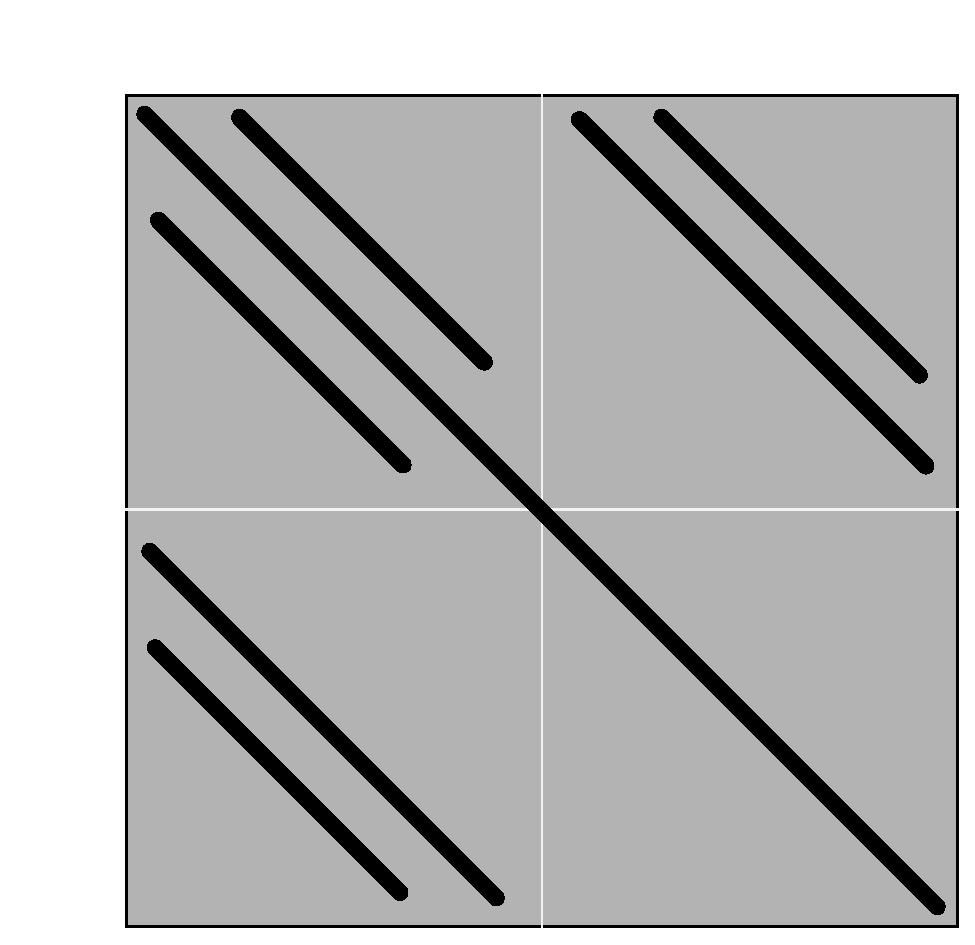
\includegraphics[width=.5\textwidth]{stateGradientsSparseMatrix.pdf}
    \caption{Schematic of sparsity structure of matrix of 2nd order gradients of internal energy with respect to states: $\ppd{\U(\pog(t),\ptg(t),\pp)}{\ptg(t)}{\ptg(t)}$. Labels at the sides correspond to $\pvg^l(t)$ and $\psg^l(t)$, i.e., each of these elements stands for a vector and thus the elements of this schematic matrix are again matrices containing the gradients defined by eqs. (\ref{eq:grad2IntActDvv}-\ref{eq:grad2IntActDuv}).}
    \label{fig:stateGrads}
\end{figure}


\subsubsection{Mixed State-Parameter Gradients}




\section{The Free Energy}
We differentiate between time-dependent (quickly varying) hidden variables (states) $\ps$ and time-independent (slowly varying) hidden variables (parameters) $\pp$.
\eq{
    \ph = \left[\begin{array}{c}
            \ps\\
            \pp
          \end{array}\right] \in \R^{n_\sh}
}

\eq{\begin{split}
    F(\po) &= \E[q(\ph)]{\log p(\po,\ph)} - \E[q(\ph)]{\log q(\ph)}\\
               &= \E[q(\ph)]{\U(\po,\ph)} + \Ent(q(\ph))
\end{split}}

In the dynamic formulation, the free energy becomes free action and falls into time-dependent and time-independent parts:
\eq{\begin{split}\label{eq:freeAction}
    \bar{F}(\Po) &= \int_0^T \E[q(\ps(t))q(\pp)]{\U(\po(t),\ps(t),\pp)}dt + \E[q(\pp)]{\U(\pp)}\\ 
    & \qquad + \int_0^T\Ent(q(\ps(t)))dt + \Ent(q(\pp))\\
    &= \int_0^T \E[q(\ps(t))q(\pp)]{\U(\po(t),\ps(t),\pp)} + \Ent(q(\ps(t))) dt\\
    & \qquad  + \E[q(\pp)]{\U(\pp)} + \Ent(q(\pp))
\end{split}}
This derives from the model:
\eq{
    p(\Po,\Ps,\pp) = p(\pp)\prod_{t=0}^T p(\po(t),\ps(t)|\pp)
}
\eq{\begin{split}\label{eq:intAction}
    \Ua(\Po,\Ps,\pp) &= \log p(\Po,\Ps,\pp)\\
    &= \log p(\pp) + \int_{t=0}^T \log p(\po(t),\ps(t)|\pp)dt\\
    &= \U(\pp) + \int_{t=0}^T \U(\po(t),\ps(t),\pp)dt
\end{split}}
where we have abused the matrix-vector notation by letting matrix formatting stand for a variable which collects values in the continuous time interval $[0,T]$ and assume that the product is defined over this continuous interval, too. The joint distribution is defined as $p(\po(t),\ps(t)|\pp) = p(\po(t)|\ps(t),\pp)p(\ps(t)|\pp)$. However, we have kept the notation as joint distribution as in \citep{Friston2008a}, because the prior $p(\ps(t)|\pp)$ is not explicitly defined there (see description of generalised filtering below). 

\section{Friston's Variational Laplace Approximation}
\subsection{Static Case}
The aim is to simplify the free energy by assuming that $q(\ph)$ is Gaussian, i.e.,
\eq{
    q(\ph) = \N(\ph|\bgs{\mu},\Cov).
}
Then, we can immediately look up the entropy of $q$ \citep[][eq. (366)]{Petersen2008} as
\eq{\begin{split}
    \Ent(q(\ph)) &= \frac{1}{2} \left(\log [2\pi^{n_\sh} \det{\Cov}] + n_\sh\right) \\
                 &= \frac{1}{2} \left(\log \det{\Cov} + n_\sh \log 2\pi e\right).
\end{split}}
The crucial trick is to approximate $\U(\po,\ph)$ (Friston calls it the internal or Gibb's energy) with a Taylor series expansion up to second order around the mean of $q$. Because the observations $\po$ are assumed to be fixed here, we drop $\po$ from the list of variables of $\U$
\eq{
    \U(\ph) \approx \U(\bgs{\mu}) + (\ph - \bgs{\mu})^\tr \U_\ph(\bgs{\mu}) + \frac{1}{2}(\ph - \bgs{\mu})^\tr \U_{\ph\ph}(\bgs{\mu}) (\ph - \bgs{\mu})
}
where $\U_\ph = \pd{\U}{\ph}$ is the gradient of $\U$ and $\U_{\ph\ph} = \ppd{\U}{\ph}{\ph}$ is the Hessian of $\U$ which are evaluated at $\bgs{\mu}$ here. We are actually interested in the expectation of $\U$
\begin{align}
    \E[q(\ph)]{\U(\ph)} &\approx 
            \E[q(\ph)]{\U(\bgs{\mu})} + \E[q(\ph)]{(\ph - \bgs{\mu})^\tr \U_\ph(\bgs{\mu})}\nonumber\\
               & \qquad + \E[q(\ph)]{\frac{1}{2}(\ph - \bgs{\mu})^\tr \U_{\ph\ph}(\bgs{\mu}) (\ph - \bgs{\mu})}\\
        &= \U(\bgs{\mu}) + \left(\E[q(\ph)]{\ph} - \bgs{\mu}\right)^\tr \U_\ph(\bgs{\mu}) + \frac{1}{2}\trace{\U_{\ph\ph}(\bgs{\mu})\Cov}\\
        &= \U(\bgs{\mu}) + \frac{1}{2}\trace{\U_{\ph\ph}(\bgs{\mu})\Cov}
\end{align}
where we have solved the expectation of the quadratic term using standard results for the multivariate Gaussian distribution \citep[][eq. (357)]{Petersen2008}. This result can be easily transferred to the case where $q$ factorises
\eq{
    q(\ph) = \prod_i q_i(\ph^i)
}
where $\ph^i \in \R^{n_{\sh_i}}$ is a subset of the hidden variables in our model, i.e., $\ph^1$ could be $\ps$ and $\ph^2$ could be $\pp$, but also further subdivisions can be used. Actually, we can still represent the factorised $q(\ph)$ with a Gaussian distribution over all variables. We just need to give $\Cov$ a suitable block-diagonal structure (assuming a suitable ordering of variables) which ensures the independence of the subsets of hidden variables $\ph^i$. These blocks of $\Cov$ are $\Cov^i$ and it is easy to see then that
\eq{\label{eq:blockq}
    \E[q(\ph)]{\U(\ph)} \approx \U(\bgs{\mu}) + \frac{1}{2}\sum_i\trace{\U_{\ph^i\ph^i}(\bgs{\mu})\Cov^i}.
}
These considerations also apply to the entropy term. Consequently, we have approximated the free energy as
\eq{\begin{split}\label{eq:FapproxC}
    F(\po) &\approx \U(\bgs{\mu}) + \frac{1}{2}\sum_i\trace{\U_{\ph^i\ph^i}(\bgs{\mu})\Cov^i} + \frac{1}{2} \sum_i\left(\log \det{\Cov^i} + n_{\sh^i} \log 2\pi e\right)\\
    &= \F(\po).
\end{split}}
Note that this is based on an approximation of $\U(\po,\ph) = \log p(\po|\ph)p(\ph) = \log p(\ph|\po) + c$ while usually the Laplace approximation is based on directly approximating the  log-posterior $\log p(\ph|\po)$. However, you see that these only differ by a constant which leads to equivalent results.

The aim of variational inference is to find $q(\ph)$ which maximises $F(\po)$ which in our case is approximated by $\F(\po)$. As $q$ is Gaussian we need to find its mean $\bgs{\mu}$ and covariance $\Cov$. Let us consider $\Cov$ first. The gradient of $\F(\po)$ with respect to $\Cov$ is\footnote{For the sake of simplicity of presentation we here ignore the potential block structure of $\Cov$, but everything goes through equivalently for any $\Cov^i$}.
\eq{
    \F_{\Cov}(\po) = \frac{1}{2} \U_{\ph\ph}(\bgs{\mu}) + \frac{1}{2} \Cov^{-1}
}
where we have used \citep[][eq. (96)]{Petersen2008} and that $\pd{\log \det{\Cov}}{\Cov} = \Cov^{-1}$ based on \citep[][eq. (43)]{Petersen2008}. Setting the gradient to 0 leads to
\eq{\label{eq:covSol}
    \Cov^{-1} = -\U_{\ph\ph}(\bgs{\mu})
}
such that
\begin{align}
    \F(\po) &= \U(\bgs{\mu}) - \frac{1}{2}\trace{\U_{\ph\ph}(\bgs{\mu})\U_{\ph\ph}^{-1}(\bgs{\mu})} + \frac{1}{2} \left(\log \det{-\U_{\ph\ph}^{-1}(\bgs{\mu})} + n_\sh \log 2\pi e\right)\nonumber\\
    &= \U(\bgs{\mu}) - \frac{1}{2}n_\sh + \frac{1}{2} \left(\log \det{-\U_{\ph\ph}^{-1}(\bgs{\mu})} + n_\sh \log 2\pi e\right)\nonumber\\
    &= \U(\bgs{\mu}) + \frac{1}{2} \left(\log \det{-\U_{\ph\ph}^{-1}(\bgs{\mu})} + n_\sh \log 2\pi\right)\\
    &= \label{eq:approxFreeE}\U(\bgs{\mu}) + \frac{1}{2} \sum_i \left(\log \det{-\U_{\ph^i \ph^i}^{-1}(\bgs{\mu})} + n_{\sh^i} \log 2\pi\right)
\end{align}
where we have reintroduced the block structure of $\Cov$ for different hidden variables in the last line.


\subsection{Dynamic Case}
We now apply these derivations in the dynamic context. We start from the free action as defined by Friston (repeated from eq. \eqref{eq:freeAction}):
\[
    \bar{F}(\Po) = \int_0^T \E[q(\ps(t))q(\pp)]{\U(\po(t),\ps(t),\pp)} + \Ent(q(\ps(t))) dt + \E[q(\pp)]{\U(\pp)} + \Ent(q(\pp)).
\]
The basic approach is to note that the parts of this equation are in the form of the static free energy above. Therefore, we can directly see from eq. \eqref{eq:FapproxC} that (remember that $\U(\pp)$ is just the prior for $\pp$ which is independent of any data)
\begin{align}
    F^\sp &= \E[q(\pp)]{\U(\pp)} + \Ent(q(\pp))\\
    &\approx \U(\bgs{\mu}_\sp) + \frac{1}{2}\trace{\U_{\pp\pp}(\bgs{\mu}_\sp)\Cov^\sp} + \frac{1}{2} \left(\log \det{\Cov^\sp} + n_{\sp} \log 2\pi e\right)\\
    &= \F^\sp.
\end{align}
Similarly, we consider the part for the states inside the integral
\begin{align}
    F^\ss(\po(t)) &= \E[q(\ps(t))q(\pp)]{\U(\po(t),\ps(t),\pp)} + \Ent(q(\ps(t)))\\
    &= \E[q(\ph)]{\U(\po(t),\ph)} + \Ent(q(\ps(t)))\\
    &\approx \U(\po(t),\bgs{\mu}) + \frac{1}{2}\trace{\U_{\ph\ph}(\po(t),\bgs{\mu})\Cov} \nonumber\\
    &\qquad + \frac{1}{2} \left(\log \det{\Cov^{\ss(t)}} + n_{\ss} \log 2\pi e\right)\\
    &= \label{eq:stateFreeAction} \U(\po(t),\bgs{\mu}_{\ss(t)},\bgs{\mu}_\sp) + \frac{1}{2}\trace{\U_{\ps(t)\ps(t)}(\po(t),\bgs{\mu}_{\ss(t)},\bgs{\mu}_\sp)\Cov^{\ss(t)}}\nonumber\\
    &\qquad + \frac{1}{2}\trace{\U_{\pp\pp}(\po(t),\bgs{\mu}_{\ss(t)},\bgs{\mu}_\sp)\Cov^\sp}\nonumber\\ 
    &\qquad + \frac{1}{2} \left(\log \det{\Cov^{\ss(t)}} + n_{\ss} \log 2\pi e\right)\\
    &= \F^\ss(\po(t))
\end{align}
where we have used the same argument as for eq. \eqref{eq:blockq} to separate the 2nd order gradients with respect to states and parameters based on their independence in $q$. Putting things together we get
\begin{align}
    \bar{F}(\Po) &= \int_0^T F^\ss(\po(t)) dt + F^\sp\\
    &\approx \int_0^T \F^\ss(\po(t)) dt + \F^\sp\\
    &= \int_0^T  \U(\po(t),\bgs{\mu}_{\ss(t)},\bgs{\mu}_\sp) + \frac{1}{2}\trace{\U_{\ps(t)\ps(t)}(\po(t),\bgs{\mu}_{\ss(t)},\bgs{\mu}_\sp)\Cov^{\ss(t)}}\nonumber\\
    &\quad + \frac{1}{2}\trace{\U_{\pp\pp}(\po(t),\bgs{\mu}_{\ss(t)},\bgs{\mu}_\sp)\Cov^\sp} + \frac{1}{2}\log \det{\Cov^{\ss(t)}} dt \nonumber\\ 
    &\quad + \U(\bgs{\mu}_\sp) + \frac{1}{2}\trace{\U_{\pp\pp}(\bgs{\mu}_\sp)\Cov^\sp}\nonumber\\
    &\quad + \frac{1}{2} \left(\log \det{\Cov^\sp} + (Tn_\ss + n_{\sp}) \log 2\pi e\right)\\
    &= \int_0^T  \U(\po(t),\bgs{\mu}_{\ss(t)},\bgs{\mu}_\sp)dt + \U(\bgs{\mu}_\sp) \nonumber\\
    &\quad + \frac{1}{2}\int_0^T \trace{\U_{\ps(t)\ps(t)}(\po(t),\bgs{\mu}_{\ss(t)},\bgs{\mu}_\sp)\Cov^{\ss(t)}}dt\nonumber\\
    &\quad + \frac{1}{2}\int_0^T \trace{\U_{\pp\pp}(\po(t),\bgs{\mu}_{\ss(t)},\bgs{\mu}_\sp)\Cov^\sp} dt + \frac{1}{2}\trace{\U_{\pp\pp}(\bgs{\mu}_\sp)\Cov^\sp}\nonumber\\
    &\quad + \frac{1}{2} \left(\int_0^T \log \det{\Cov^{\ss(t)}} dt + \log \det{\Cov^\sp} + (Tn_\ss + n_{\sp}) \log 2\pi e\right)\\
    &= \label{eq:approxFreeActionFull} \int_0^T  \U(\po(t),\bgs{\mu}_{\ss(t)},\bgs{\mu}_\sp)dt + \U(\bgs{\mu}_\sp) \nonumber\\
    &\quad + \frac{1}{2}\int_0^T \trace{\U_{\ps(t)\ps(t)}(\po(t),\bgs{\mu}_{\ss(t)},\bgs{\mu}_\sp)\Cov^{\ss(t)}}dt\nonumber\\
    &\quad + \frac{1}{2} \trace{\left(\int_0^T \U_{\pp\pp}(\po(t),\bgs{\mu}_{\ss(t)},\bgs{\mu}_\sp)dt + \U_{\pp\pp}(\bgs{\mu}_\sp)\right)\Cov^\sp}\nonumber\\
    &\quad + \frac{1}{2} \left(\int_0^T \log \det{\Cov^{\ss(t)}} dt + \log \det{\Cov^\sp} + (Tn_\ss + n_{\sp}) \log 2\pi e\right)\\
    &= \Fa(\Po).
\end{align}
In analogy to eq. \eqref{eq:covSol} we see that the posterior state covariances which maximise $\Fa(\Po)$ are given as
\eq{\label{eq:postCovStates}
    \Cov^{\ss(t)^{-1}} = -\U_{\ps(t)\ps(t)}(\po(t),\bgs{\mu}_{\ss(t)},\bgs{\mu}_\sp).
}
Equivalently, we can derive the posterior parameter covariance:
\eq{\label{eq:postCovParam}
    \Cov^{\sp^{-1}} = -\left(\int_0^T \U_{\pp\pp}(\po(t),\bgs{\mu}_{\ss(t)},\bgs{\mu}_\sp)dt + \U_{\pp\pp}(\bgs{\mu}_\sp)\right).
}
Plugging in the result for the posterior state covariance we can simplify eq. \eqref{eq:approxFreeActionFull} as above
\begin{align}
    \Fa(\Po) &= \label{eq:approxFreeAction} \int_0^T  \U(\po(t),\bgs{\mu}_{\ss(t)},\bgs{\mu}_\sp)dt +  \U(\bgs{\mu}_\sp) \nonumber\\
    &\quad + \frac{1}{2} \left(\int_0^T \log \det{\Cov^{\ss(t)}} dt + \log \det{\Cov^\sp} + (Tn_\ss + n_{\sp}) \log 2\pi\right).
\end{align}


\section{Finding the Posterior Mode of the Parameters}
It is now tempting to implement the parameter learning by gradient ascent on $\Fa(\Po)$ with respect to the posterior mode of the parameters $\bgs{\mu}_\sp$. The gradient of the approximated free action is (for simplicity of treatment we consider only a single parameter $\mu_{\sp_i}$):
\begin{align}
    \Fa_{\mu_{\sp_i}}(\Po) &= \Ua_{\sp_i}(\Po,\bgs{\mu}_\Ps,\bgs{\mu}_\sp) + \frac{1}{2}\int_0^T \trace{\U_{\ps(t)\ps(t)\sp_i}(\po(t),\bgs{\mu}_{\ss(t)},\bgs{\mu}_\sp)\Cov^{\ss(t)}}dt\nonumber\\
    &\quad \label{eq:approxFreeActionDp} + \frac{1}{2}\trace{\Ua_{\pp\pp\sp_i}(\Po,\bgs{\mu}_\Ps,\bgs{\mu}_\sp)\Cov^\sp}.
\end{align}
We derived this gradient using 
\begin{align}
    \pd{\log \det{\Cov}}{x} &= \frac{1}{\det{\Cov}}\det{\Cov}\trace{\Cov^{-1}\pd{\Cov}{x}}\\
    &= \trace{\Cov^{-1}\Cov\pd{\bs{U}}{x}\Cov}\\
    &= \trace{\pd{\bs{U}}{x}\Cov}
\end{align}
together with $\Cov = -\bs{U}^{-1}$ based on \citep[][eqs. (41) and (53)]{Petersen2008}. The second order gradients with respect to $\sp_j$ can be derived using
\begin{align}
    \pd{\pd{\bs{U}}{x}\Cov}{y} &= \ppd{\bs{U}}{x}{y}\Cov - \pd{\bs{U}}{x}\pd{\bs{U}^{-1}}{y}\\
    &= \ppd{\bs{U}}{x}{y}\Cov + \pd{\bs{U}}{x}\bs{U}^{-1}\pd{\bs{U}}{y}\bs{U}^{-1}\\
    &= \ppd{\bs{U}}{x}{y}\Cov + \pd{\bs{U}}{x}\Cov\pd{\bs{U}}{y}\Cov
\end{align}
what leads to
\begin{align}
    \Fa_{\mu_{\sp_i}\mu_{\sp_j}}(\Po) &= \Ua_{\sp_i\sp_j}(\Po,\bgs{\mu}_\Ps,\bgs{\mu}_\sp) \nonumber\\
    &\quad + \frac{1}{2}\int_0^T \trace{\U_{\ps(t)\ps(t)\sp_i\sp_j}\Cov^{\ss(t)} - \U_{\ps(t)\ps(t)\sp_i}\Cov^{\ss(t)}\U_{\ps(t)\ps(t)\sp_j}\Cov^{\ss(t)}} dt\nonumber\\
    &\quad \label{eq:approxFreeActionDpDp} + \frac{1}{2}\trace{\Ua_{\pp\pp\sp_i\sp_j}\Cov^\sp + \Ua_{\pp\pp\sp_i}\Cov^\sp\Ua_{\pp\pp\sp_j}\Cov^\sp}
\end{align}
where we have dropped the dependencies of $\U$ for convenience of writing. However, these gradients also depend on the posterior modes of the states $\bgs{\mu}_\Ps$ and maximisation of $\Fa(\Po)$, therefore, will have to iterate between maximising posterior modes of states and posterior modes of parameters.

It is clear now that we need third and fourth order gradients of $\U$ to maximise $\Fa(\Po)$ which makes this optimisation computationally very expensive. For example, to compute all elements of the matrix defined by $[\cdot]_{ij} = \trace{\Ua_{\pp\pp\sp_i}\Cov^\sp\Ua_{\pp\pp\sp_j}\Cov^\sp}$ is of complexity $O(n_\sp^6)$ where $\pp \in \R^{n_\sp\times 1}$ (when ignoring the cost of computing the gradients of $\Ua_{\pp\pp}$). Similarly, computing all elements defined by the second line of eq. \eqref{eq:approxFreeActionDpDp} has complexity $O(n_\sp^2n_\ss^4)$. Computing the first order gradient $\Fa_{\pp}(\Po)$ still has complexity $O(n_\sp n_\ss^2)$, or $O(n_\sp^3)$, respectively, depending on whether $n_\ss$ or $n_\sp$ is larger.

Friston finds the posterior mode in a different way. Equivalently to the dynamic solution for the states he uses the variational result that $\bar{F}(\Po)$ is maximised with respect to $q(\pp)$, while holding $q(\Ps)$ fixed, when
\eq{\label{eq:qParamVariational}
    q(\pp) = \frac{1}{Z^\sp} \exp(\Va(\Po,\pp))
}
where
\begin{align}
    \Va(\Po,\pp) &= \E[q(\Ps)]{\Ua(\Po,\Ps,\pp)}\\
    &= \U(\pp) + \int_0^T \E[q(\ps(t))]{\U(\po(t),\ps(t),\pp)} dt\\
    &\approx \U(\pp) + \int_0^T \U(\po(t),\bgs{\mu}_{\ss(t)},\pp) dt \nonumber\\
    &\quad + \frac{1}{2}\int_0^T \trace{\U_{\ps(t)\ps(t)}(\po(t),\bgs{\mu}_{\ss(t)},\pp)\Cov^{\ss(t)}} dt\\
    &= \label{eq:approxVarAction} \Ua(\Po,\bgs{\mu}_\Ps,\pp) + \frac{1}{2}\int_0^T \trace{\U_{\ps(t)\ps(t)}(\po(t),\bgs{\mu}_{\ss(t)},\pp)\Cov^{\ss(t)}}dt
\end{align}
where we have used the independence of the $q(\ps(t))$ and the first line of eq. \eqref{eq:stateFreeAction} (a result from the Laplace approximation). We only need to find the (rather "a") mode of $q(\pp)$ from which we already can compute $\Cov^\sp$ (provided we also have the modes $\bgs{\mu}_{\ss(t)}$) which would complete our Laplace approximation. Also, it is clear from eq. \eqref{eq:qParamVariational} that a maximum of $q(\pp)$ (a mode) is equal to a maximum of $\Va(\Po,\pp)$, because the exponential function is monotonically increasing. Hence, Friston suggests to maximise $\Va(\Po,\pp)$ instead of directly maximising $\Fa(\Po)$. At this point it is instructive to remember that the interpretation of the two optimisations is different. We maximise $\Fa(\Po)$ directly with respect to the posterior mode $\bgs{\mu}_\sp$ which was possible because of the Laplace approximation for both states and parameters. On the other hand, we maximise $\Va(\Po,\pp)$ with respect to the parameters used in the model $\pp$ in order to find a posterior mode $\bgs{\mu}_\sp$ based on a Laplace approximation around the posterior mode of the states only. Notice that this approach makes no assumptions about the form of $q(\pp)$ while we assumed a Gaussian $q(\pp)$ in deriving $\Fa(\Po)$.

The first and second order gradients of $\Va(\Po,\pp)$ are
\begin{align}
    \Va_{\sp_i}(\Po,\pp) &= \label{eq:approxVarActionDp} \Ua_{\sp_i}(\Po,\bgs{\mu}_\Ps,\pp) + \frac{1}{2}\int_0^T \trace{\U_{\ps(t)\ps(t)\sp_i}(\po(t),\bgs{\mu}_{\ss(t)},\pp)\Cov^{\ss(t)}}dt
\end{align}
\begin{align}
    \Va_{\sp_i\sp_j}(\Po,\pp) &= \label{eq:approxVarActionDpp} \Ua_{\sp_i\sp_j}(\Po,\bgs{\mu}_\Ps,\pp) + \frac{1}{2}\int_0^T \trace{\U_{\ps(t)\ps(t)\sp_i\sp_j}(\po(t),\bgs{\mu}_{\ss(t)},\pp)\Cov^{\ss(t)}}dt.
\end{align}
Therefore, this approach saves us the computation of $\frac{1}{2}\trace{\Ua_{\pp\pp\sp_i}(\Po,\bgs{\mu}_\Ps,\bgs{\mu}_\sp)\Cov^\sp}$ in the first order gradients (compare eqs. \ref{eq:approxFreeActionDp} and \ref{eq:approxVarActionDp}) and also considerably simplifies computation of the second order gradients. 

Shouldn't both approaches lead to a mode $\bgs{\mu}_\sp$ which maximises $\Fa(\Po)$? Eventually, i.e., after iterating between optimising for $\bgs{\mu}_\sp$ and optimising for $\bgs{\mu}_\Ps$, we guess, yes, but this is hard to see from these equations. We do note, though, that optimising $\Fa(\Po)$ with respect to $\bgs{\mu}_\sp$ takes additionally the posterior uncertainty $\Cov^\sp$ of $\pp$ (which is a function of $\bgs{\mu}_\sp$) into account while this only enters in the computation of the posterior mode $\bgs{\mu}_\Ps$ in the variational approach. Potential advantages of this, e.g., in terms of better convergence properties, are unclear to us at this point.

The computational advantage of optimising $\Va(\Po,\pp)$ instead of $\Fa(\Po)$ is greatest for the second order gradients where the complexity for computing all elements of $[\cdot]_{ij} = \trace{\U_{\ps(t)\ps(t)\sp_i\sp_j}(\po(t),\bgs{\mu}_{\ss(t)},\pp)\Cov^{\ss(t)}}$ is $O(n_\sp^2n_\ss^2)$. Nevertheless, 4th order gradients of $\Ua$ still need to be computed. We could radically reduce the computational costs further, if we ignore the mean-field terms of the variational approximation. Then, the gradients simply become
\begin{align}
    \Va_{\sp_i}(\Po,\pp) &= \Ua_{\sp_i}(\Po,\bgs{\mu}_\Ps,\pp)
\end{align}
\begin{align}
    \Va_{\sp_i\sp_j}(\Po,\pp) &= \Ua_{\sp_i\sp_j}(\Po,\bgs{\mu}_\Ps,\pp)
\end{align}
and we would have reduced our variational problem to a simple maximum a posteriori optimisation to find the mode of our approximated posterior density $q(\pp)$. In this case, the only computational complexity left would be the cost of computing the first and second order gradients of $\Ua$. This is actually what would usually be understood as the Laplace approximation: find the MAP estimate for $\pp$ and then simply put a Gaussian around it based on the local curvature of $\Ua$ (cf. eq. \eqref{eq:postCovParam}). Of course, when using this approach, we would ignore the uncertainty of the states and the result would not be a solution which optimises the approximated free action $\Fa(\Po)$ anymore. On the other hand, this may still be a viable approach when the uncertainties are low such that the mean-field terms contribute only little to the optimisation.

In conclusion, we have presented three approaches to finding an approximated posterior mode of parameters $\bgs{\mu}_\sp$ which, for the benefit of decreasing computational costs, take decreasing amounts of information about posterior uncertainty of states and parameters into account.


\section{Following the Posterior Mode of the States}
We now come to the core of Friston's approach to filtering. We believe that his derivation based on an ensemble of particles is confusing and unnecessary. We will ignore it and take a more direct approach. The main idea is the following: View finding the mode of a distribution as gradient ascent in a dynamical system, extend this to the case where the mode underlies a constant drift and show that a representation in generalised coordinates can estimate that drift.

Before, we have seen that the variational posterior is a function of the variational energy, i.e., holding $q(\pp)$ fixed, the approximated posterior for the states at time $t$ is (\todo this needs to be shown for $\ps(t)$ cf. $\Ps$)
\eq{
    q(\ps(t)) = \frac{1}{Z^{\ss(t)}}\exp\left(\V(\Po,\ps(t)) \right).
}
Let us now replace the time-varying $\ps(t)$ with a variable which is constant across time: $\ps(t)=\ph$
\eq{
    q(\ph) = \frac{1}{Z^{\sh}}\exp\left(\V(\Po,\ph) \right).
}
Hence, a mode of $q(\ph)$ is also a maximum of $\V(\Po,\ph)$. One way of finding such a maximum is to do gradient ascent on $\V$ which may be formulated in continuous time as
\eq{\label{eq:dynGradientAscent}
    \frac{\ud \ph}{\ud t'} = \ph' = \pd{\V(\Po,\ph)}{\ph}.
}
To make this explicit: this dynamical system will follow the gradient of $\V$ until it reaches a maximum of $\V$ (equal to $\ppm_{\ss(t)}$) at which $\ph'=0$, i.e., maxima of $\V$ are stable fixed points of this dynamical system while minima are unstable fixed points. Notice that this dynamical system operates in a different time frame $t'$ than the real time $t$ above. In other words, in the new time frame the posterior mode $\ppm_{\ss(t)}$ is constant. This is obviously wrong. So we introduce a drift variable $\ph'^*$ which is constant in the frame of $t'$ and is supposed to represent the change of the posterior mode in real time $t$
\eq{
    \ph' = \pd{\V(\Po,\ph)}{\ph} + \ph'^*.
}
The difference between the time frames is only a theoretical construct, because they actually evolve simultaneously. Hence, when we are at a maximum of $\V$ with $\ph=\ppm_{\ss(t)}$
\eq{
    \ph' = \ph'^*,
}
i.e., the change in $\ph$ actually tracks the change in the posterior mode $\ppm_{\ss(t)}$, if we can ensure that $\ph'^* = \dot{\ppm}_{\ss(t)}$. The trick now is to use generalised coordinates to simultaneously approximate $\ppm_{\ss(t)}$ and $\dot{\ppm}_{\ss(t)}$. We do this by setting up two (or more) simultaneous dynamical systems:
\begin{align}
    \label{eq:generalisedpostmodepos} \ph' &= \pd{}{\ph}\V(\Po,\ph,\ph',\dots) + \ph'^*\\
    \label{eq:generalisedpostmodevel} \ph'' &= \pd{}{\ph'}\V(\Po,\ph,\ph',\dots) + \ph''^*\\
    \vdots \nonumber
\end{align}
where we define $\ph'' = \ud \ph' / \ud t''$ and denote the current state of the dynamical system defined by $\ph''$ in eq. \eqref{eq:generalisedpostmodevel} as $\ph'^*$ to differentiate it from $\ph'$ in eq. \eqref{eq:generalisedpostmodepos} (similarly for higher order generalised coordinates). Now remember that (in our new notation) $\ph^* = \ps(t)$ and correspondingly $\ph'^* = \dot{\ps}(t)$. We also know that the dynamical systems for $\ph'$ and $\ph''$ converge to $\ppm_{\ss(t)}$ and $\dot{\ppm}_{\ss(t)}$, respectively, when the contribution from the higher order coordinates is ignored. Hence, $\ph'^* = \dot{\ppm}_{\ss(t)}$ after convergence and will provide the drift of the posterior mode (which may be influenced by the drift of the drift of the posterior mode as estimated by the next higher coordinate, and so on). 

It is possible to write these equations more compactly by using generalised coordinate notation:
\eq{\label{eq:Dstepdynamics}
    \dot{\phg} = \pd{\V(\Po,\phg)}{\phg} + \D\phg
}
where $\D$ is the matrix derivative operator which shifts coordinates up as defined in eq. \eqref{eq:derivativeOperator}. Note that all the dynamical systems now are formulated in a common time frame again. This does not change anything, because we only introduced the different time frames as an aid to understand the working of the combined system. But does the combined dynamical system now actually converge to $\ppmg_{\ss(t)}$? Friston provides a linear stability analysis around the posterior mode $\ppmg_{\ss(t)}$. This does not add much to what we already know from the previous considerations, but for completeness we repeat it anyway:

Make a first-order Taylor approximation of the variational energy gradient around the mode
\eq{\begin{split}
    \pd{\V(\Po,\phg)}{\phg} &= \pd{\V(\Po,\ppmg_{\ss(t)})}{\phg} + (\phg - \ppmg_{\ss(t)})^\tr \ppd{\V(\Po,\ppmg_{\ss(t)})}{\phg}{\phg}\\
    &= \pd{\V(\Po,\ppmg_{\ss(t)})}{\phg} + \bgs{\varepsilon}^\tr \ppd{\V(\Po,\ppmg_{\ss(t)})}{\phg}{\phg}\\
    &=\bgs{\varepsilon}^\tr \ppd{\V(\Po,\ppmg_{\ss(t)})}{\phg}{\phg}
\end{split}}
where we have used $\pd{\V(\Po,\phg)}{\phg} = 0$ for $\phg = \ppmg_{\ss(t)}$ on the last line. Plug into eq. \eqref{eq:Dstepdynamics}
\eq{\begin{split}
    \dot{\phg} &= \bgs{\varepsilon}^\tr \ppd{\V(\Po,\ppmg_{\ss(t)})}{\phg}{\phg} + \D\phg\\
   &= \bgs{\varepsilon}^\tr \ppd{\V(\Po,\ppmg_{\ss(t)})}{\phg}{\phg} + \D (\bgs{\varepsilon} + \ppmg_{\ss(t)}).
\end{split}}
Use $\dot{\ppmg}_{\ss(t)} = \D\ppmg_{\ss(t)}$
\begin{align}
    \dot{\phg} &= \bgs{\varepsilon}^\tr \ppd{\V(\Po,\ppmg_{\ss(t)})}{\phg}{\phg} + \D\bgs{\varepsilon} + \dot{\ppmg}_{\ss(t)}\\
    \dot{\bgs{\varepsilon}} &= \bgs{\varepsilon}^\tr \ppd{\V(\Po,\ppmg_{\ss(t)})}{\phg}{\phg} + \D\bgs{\varepsilon}\\
    &= \left(\left[\ppd{\V(\Po,\ppmg_{\ss(t)})}{\phg}{\phg}\right]^\tr + \D\right) \bgs{\varepsilon}\\
    &= \left(\V_{\phg\phg}^\tr + \D\right) \bgs{\varepsilon}
\end{align}
The resulting dynamical system of the difference between $\phg$ and the posterior mode $\bgs{\varepsilon} = \phg - \ppmg_{\ss(t)}$ is a simple linear system which converges to $\bs{0}$ exponentially fast as long as $\V_{\phg\phg}^\tr + \D$ is negative definite. We know that $\V_{\phg\phg}$ has a negative effect, because we are close to a maximum of $\V(\Po,\phg)$ and the curvature there is negative. Hence, whether $\phg$ converges to $\ppmg_{\ss(t)}$ depends on whether $\V_{\phg\phg}$ dominates over $\D$. Friston suggests to scale $\V_{\phg\phg}$ by a constant to ensure that the contribution of $\V_{\phg\phg}$ is sufficiently large, but notes that this was unnecessary in their experience. Overall this analysis provides little more information than our original insight that the dynamical system in eq. \eqref{eq:dynGradientAscent} converges to $\ppm_{\ss(t)}$.

In summary, the main filtering equation in Friston's DEM is eq. \eqref{eq:Dstepdynamics}. For a static system the solution of the variational approximation ensures that the dynamical system defined by eq. \eqref{eq:Dstepdynamics} converges to a mode of the variational posterior distribution. In a dynamic setting, where this mode moves itself, the representation in generalised coordinates ensures that the whole movement of the mode is estimated. The differential term $\D\phg$ is important, because it ensures that the estimate of the mode in one coordinate has the appropriate effect for tracking the mode in the next lower-order coordinate (e.g. the estimated velocity of the mode is taken into account when tracking the mode itself given an observation). 


\section{Discretisation}
For an actual implementation we have to discretise the time integrals in this equation. One straightforward way of doing this is to simply use the time points at which we observed the data points $\po(t)$, but note that with the transformation into generalised coordinates the discretisation can be done independently from the observations and may, therefore, be made more precise, if necessary. Without loss of generality we from here assume that a discretisation step is the size of a time unit such that the approximated free action becomes
\begin{align}
    \Fa(\Po) &= \label{eq:approxFreeActionDisc} \U(\bgs{\mu}_\sp) + \sum_{t=0}^T  \U(\po(t),\bgs{\mu}_{\ss(t)},\bgs{\mu}_\sp) \nonumber\\
    &\quad + \frac{1}{2} \left(\log \det{\Cov^\sp} + (Tn_\ss + n_{\sp}) \log 2\pi + \sum_{t=0}^T \log \det{\Cov^{\ss(t)}}\right).
\end{align}


\bibliographystyle{ieeetr}
\bibliography{DEMpapers}

\end{document}
